\chapter{Conceitos Preliminares}
\label{FundamentacaoTeorica}
%%
%Exemplo de referência bibliográfica \cite{abntex2-wiki-como-customizar}.

%Exemplo de uso de figura no Latex (Figura~\ref{fig:mafalda}).
%\begin{figure}[th]
%\centering{
%\caption{Legenda da Figura no topo.}
%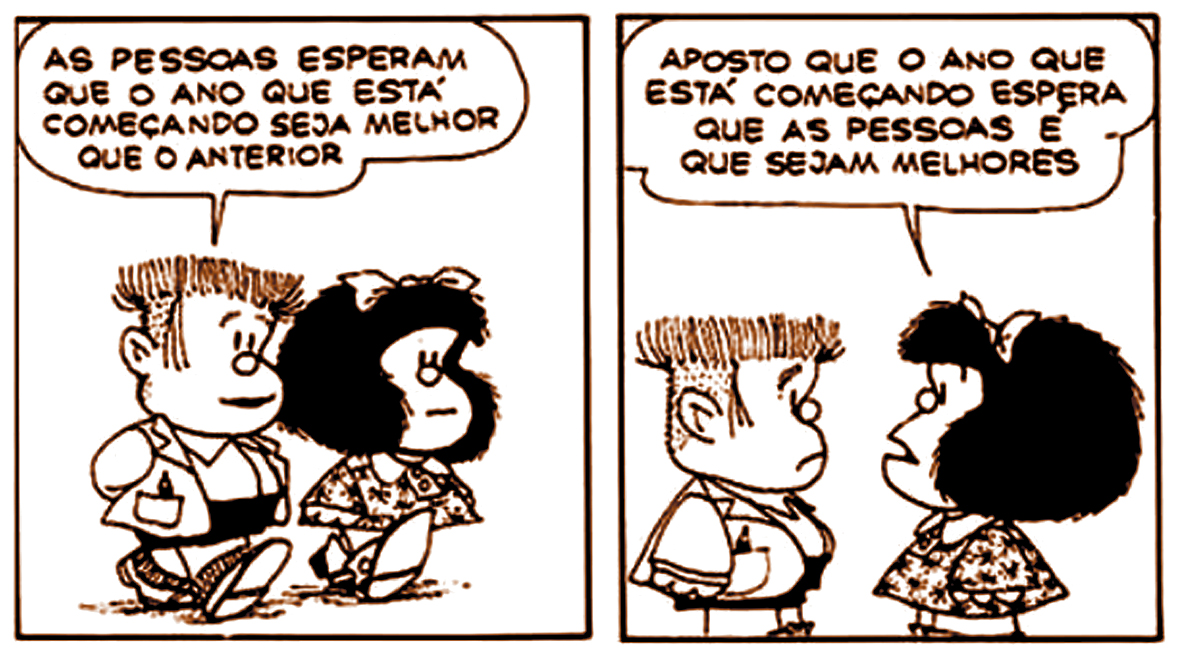
\includegraphics[width=0.75\textwidth]{figuras/mafalda}
%\begin{flushleft}
%\flushleft{Fonte: 
%Elaborado pelo autor.}
%\end{flushleft}
%\label{fig:mafalda}
%}
%\end{figure}


%Exemplo de uso de tabela no Latex (Tabela~\ref{tab:tabelaModelo}). Ver página 72 do Manual de Normalização de Trabalhos Acadêmicos do IFCE.
%\begin{table}[th]
%\centering
%\caption{Legenda da Tabela no Topo.}
%\label{tab:tabelaModelo}
%\begin{tabular}{llll}
%& Nota mínima & Nota máxima & Nota média\\\hline
%Ciências Humanas (CH)     & 324,8       & 862,1       & 546,5\\
%Ciências da Natureza (CN) & 330,6       & 876,4       & 482,2\\
%Linguagens e Códigos (LC) & 306,2       & 814,2       & 507,9\\
%Matemática (MT)           & 318,5       & 973,6       & 473,5\\ \hline  
%\end{tabular}
%\begin{flushleft}
%\flushleft{Fonte: 
%Instituto Brasileiro de Geografia e Estatística - IBGE.}
%\end{flushleft}
%\end{table}

Nessa subseção veremos uma  breve explicação de conceitos preliminares e tecnologias utilizadas. Isso será necessário para uma melhor compreensão dos Trabalhos Relacionados. 


\section{ Conceitos Teóricos }
Pode-se organizar o software de um jogo, num primeiro momento, em uma hierarquia de telas (screens). Assim, ao entrar num jogo, pode-se apresentar num determinado ponto uma tela inicial com um menu de opções (menu screen). O usuário poderá fazer algumas escolhas e configurações nesse momento inicial do jogo e depois escolher uma opção para iniciar o jogo, quando então se parte para a tela principal(main screen). Visualmente, pode-se realizar uma transição de uma tela para a outra (screen transition); existem diferentes animações gráficas para realizar esse tipo de transição, que normalmente envolve um movimento de saída da tela atual e o movimento de entrada da tela seguinte.

Uma vez na tela principal do jogo, geralmente há uma imagem de fundo (background image) que dá forma ao tabuleiro do jogo (board). O tabuleiro pode ser considerado como uma estrutura gráfica onde ocorre a “ação” propriamente dita do jogo. Há formas de construir a imagem do tabuleiro ou do fundo através de unidades gráficas menores chamadas de tiles. Os jogadores e demais personagens animados que possam haver no jogo são representados por objetos gráficos que se movem pelo cenário, sendo chamados de sprites. O movimento dos sprites que representam os jogadores tipicamente ocorre por um caminho pré-definido de posições no tabuleiro que será definido aqui como path.
Às vezes, o tabuleiro é grande demais para caber inteiramente de uma vez na tela. Nesse caso, pode-se focar somente uma certa área parcial do tabuleiro na tela. A área do tabuleiro que aparece na tela é controlada em função da posição da câmera. Assim, jogos gráficos com tabuleiros maiores poderão executar sem problemas mesmo em telas menores.

Geralmente, jogos de tabuleiro, por apresentarem uma dinâmica mais simples, apresentam os seus principais dados na tela, em painéis que indicam os pontos dos jogadores, isto é, o score da partida. Além disso, precisa ser indicado na tela de quem é o turno atual de jogada, já que nesses jogos a execução é tipicamente encadeada na forma de turnos (turn-based games). Pode-se chamar de estado atual do jogo (game state) o conjunto completo dessas informações: de qual jogador é o turno atual,todas as pontuações de cada jogador, a posição de cada um no tabuleiro e demais variáveis que controlam a situação atual do jogo.

Durante o jogo, a interface gráfica contará principalmente com movimentos dos sprites sobre o tabuleiro e eventuais caixas de diálogo (dialogs). Essas caixas de diálogo guiam o processo do jogo. No caso de jogos educativos de tabuleiro, podem trazer uma pergunta, as possibilidades de resposta do jogador, etc. Em muitos jogos, há o uso de algum tipo de fator aleatório para guiar o movimento do jogador,tipicamente realizado com a jogada de um dado (dice). Isso pode ser apresentado na forma de uma caixa de diálogo também.

Convém lembrar que a interface gráfica de muitos jogos é tipicamente controla via teclado. No caso de jogos para Web, é frequente a opção de controle por mouse também. Assim, deve-se ter o cuidado, em cada tela, de poder responder tanto pelo teclado quanto pelo mouse na medida em que isso for possível. No caso de uma tela de menu, pode-se ter um indicador visual (cursor) para definir em qual opção o usuário está atualmente selecionado. Caso o usuário simplesmente clique com o mouse numa outra opção, o cursor é colocado imediatamente ali e então a opção é ativada. Assim, mantém-se a devida harmonia no uso da aplicação.

Por fim, quando o jogo termina, uma tela final pode ser apresentada (ending screen). Nessa tela,tipicamente são apresentados os pontos finais de cada um e algumas estatísticas sobre a partida, como tempo ou número de acertos, erros, movimentos de um tipo ou outro, ou qualquer outra possibilidade de informação conforme admita o tipo do jogo.

Em toda a execução do jogo, do início ao fim, pode-se pressupor algum tipo de música de fundo(background music), com sons adicionais para cada ação (sounds), enriquecendo a experiência do jogador.

Uma observação que se sobressai diante da análise desses conceitos é que há uma estrutura relativamente comum a muitos jogos do gênero; essa estrutura não necessitaria, a princípio, de ter que ser completamente descrita por programação de código. Seria possível descrever parte dessa estrutura por meio de uma descrição mais simples, apropriada para uma automatização do desenvolvimento de jogos. Isso, de fato, é uma das contribuições do presente trabalho, que permitirá, conforme será visto mais adiante, descrever partes da estrutura do jogo como uma descrição textual num arquivo de simples personalização. Isso facilita a utilização do \textit{framework} proposto por outros educadores brasileiros que possam ter um conhecimento menos profundo na área de jogos, para que possam mais rapidamente montar um jogo que sirva ao propósito de diversão com aprendizado e enriquecimento cultural.

 \subsection{ Bitmap }

 O Bitmap é um formato padrão de imagem que contém uma matriz de \textit{pixels}, fornecendo a cor de cada pixel. Não contém informações geométricas sobre os objetos que estariam compondo a imagem, mas apenas a cor em cada pixel. Assim, esse formato não permite que a imagem possa ser esticada de forma a preservar as descrições geométricas dos objetos desenhados. É usado para fotos e outros tipos de desenho em que não é necessário esticar ou manipular partes.

\section{Conceitos Tecnológicos}

Considerando a proposta de desenvolvimento de jogos gráficos que utilizam tecnologias da Web, esta seção irá explicar algumas das principais tecnologias envolvidas nesse contexto. Algumas tecnologias no contexto de desenvolvimento na Web são opcionais: o desenvolvedor pode ou não utilizá-la. Os casos que foram avaliados como de uso mais frequente no desenvolvimento de jogos ou ainda que possam ter relevância perante o \textit{framework} sendo proposto neste trabalho foram selecionados para breves explicações aqui. Para maiores informações sobre cada uma das tecnologias sendo descritas à seguir, algumas referências são também apresentadas para o leitor consultar.

\subsection{ HTML }
 O HTML (Hypertext Markup Language) é a linguagem de marcação padrão de documentos que foram criados para serem exibidos em navegadores na Web. Ela é formada por blocos chamados \textit{tags}, esses blocos dão significado semântico ao conteúdo do documento, como por exemplo, a \textit{tag} 'p' dá o significado semântico de parágrafo ao conteúdo dentro dela, o conteúdo das \textit{tags} pode variar de texto, imagem e vídeo \cite{musciano1996html}.
 
 \subsection{ XML }
 
 %#4
 A Extensible Markup Language (XML), faz parte das SGMLs (Standard Generalized Markup Language), é um padrão para documentos de linguagens genéricas de marcação. Foi criada em 1998 pela XML Working Group, com o objetivo de ser usado diretamente na internet. Tecnicamente um documento XML é formado por entidades que podem se referir a outras entidades, sendo uma destas a entidade raiz, desta forma representando informações em um esquema similar a um grafo \cite{bray2000extensible}.
 
 \subsection{ CSS }

CSS  (Cascading Style Sheets) pode ser usada em conjunto com o HTML para descrever  como as informações contidas nas
\textit{tags} serão apresentadas. Ela foi criada para separar o conteúdo do estilo, cuidando de informações como
cores, posicionamento do conteúdo na página e quais
fontes usar para cada texto. Essa separação pode
ajudar na
acessibilidade e permitir flexibilidade às
páginas Web \cite{ahmadian2011desnutrin}.

 \subsection{ Javascript }

O Javascript é uma linguagem de programação de \textit{script} interpretada, como elementos de programação
orientada a objeto, criada com o objetivo de
tornar a página \textit{Web} dinâmica, definindo
seu comportamento e possibilitando a
interatividade com usuário
\cite{flanagan2006javascript}. Ela interage
diretamente com os outros pilares da
\textit{World Wide Web}: CSS e HTML.

\subsection{ Typescript }

O Typescript é uma linguagem que expande JavaScript. Foi criada com o objetivo de fazer o desenvolvimento de \textit{software} usando Javascript mais fácil em grandes escalas. Além disso essa extensão também possui alguns recursos que podem ser, com frequência, interessantes para um desenvolvedor, como tipagem de variáveis \cite{bierman2014understanding}.

 \subsection{ SVG }
 
 SVG  (Scalable Vector Graphics) é um formato de imagem vetorial para gráficos 2D baseado em XML  (Extensible Markup Language), uma linguagem de marcação
 \cite{ferraiolo2000scalable}. Ele possui suporte
 a interatividade e animações. Esse formato foi
 criado pela W3C (World Wide Web Consortium) desde
 1999 \cite{ferraiolo2000scalable}. O SVG pode se
 integrar às páginas Web através do HTML, com uso
 da \textit{tag} 'svg', oficialmente adicionada
 no HMTL5, os atributos pode ser estilizados
 através do CSS, como qualquer outro elemento de
 html5, e como uso do Javascript é possível criar animação e eventos interativos.
 
\subsection{ Canvas }
 
Canvas é um dos elementos do HTML que permite a renderização dinâmica de formas e  imagens \textit{bitmap}. Ele também
permite desenhar objetos 3D, com auxilio da WebGL (Web Graphics Library), uma biblioteca para renderização de gráficos 2D e 3D
no contexto das páginas Web \cite{shappir2012performing}.

\chapter{Frameworks de Jogos para Web}

\section{Delimitação da Pesquisa}

Conforme mencionado na Introdução, pretende-se trabalhar com jogos leves de tabuleiro. Nisso o presente trabalho pressupõe o gênero 2D de jogos gráficos, que é o mais frequente para esse tipo de jogo.Além disso, é desejável aqui que o jogo possa executar em uma variedade de sistemas computacionais,sem exigência de um equipamento mais caro. Isso significa que a natureza de jogo pretendida é tal que não se imponha o uso de uma CPU de última geração, ou grande quantidade de memória no sistema ou ainda uma GPU mais avançada. Portanto, o foco da pesquisa fica delimitado a uma execução mais leve no Browser. Observação: o termo “leve” pode ser considerado subjetivo – o que é leve para um usuário pode não ser leve para outro. Porém, a natureza gráfica 2D mais simples de jogos de tabuleiro já torna essa categorização mais simples, conforme se poderá inferir da própria apresentação dos frameworks à seguir.

\section{Framewroks}

\subsection{ Phaser }

Desenvolvido pela Photon Storm, Phaser é um
\textit{framework} gratuito e \textit{
open-source } para o desenvolvimento de jogos 2D
HTML5. Ele usa renderização com Canvas ou WebGL e
pode trocar entre eles automaticamente dependendo
do suporte do  \textit{browser}. Pode ser
compilado para IOS (iPhone Operating System),
Android e aplicações nativas com o uso de
\textit{Third-party software}, o desevolvedor
pode usar tanto Javascript como também Typescript
\cite{faas2017introduction}. 

O Phaser possuir um bom \textit{design}, é bem documentado, possui suporte e foi criado em com base no PixiJS, que será abordado posteriormente. Portanto, os principais problemas deste \textit{framework} são muitas vezes referentes à linguagem Javascript, para a qual o \textit{framework} for desenvolvido, fazendo com que frequentemente os desenvolvedores usem Typescript.

\subsection{ PixiJS }

O PixiJS (Pixi Javascript) é uma biblioteca, com estrutura de código muito similar ao ActionScript, de renderização que permite criar gráficos ricos e interativos, aplicações para múltiplas plataformas  e jogos sem a necessidade de um conhecimento profundo na WebGL ou lidar com compatibilidade de navegador e dispositivo. Caso o WebGL não seja suportado por alguma razão, o PixilJS é capaz de trocar para o uso do Canvas. Ela se torna uma biblioteca atrativa para usuários de ActionScript, por sua similaridade de estrutura. Segundo a Goodboy, empresa que o criou \cite{van2015learn}, o PixiJs tem como principal vantagem, a velocidade de renderização que faz com que muitas vezes ela seja utilizada por outros \textit{frameworks} com Phaser por exemplo \cite{van2015learn}.
Essa biblioteca realiza bem o que se propõe, renderização, mas apenas isso pode ser visto como muito pouco, na criação de jogos, em comparação a outros trabalhos também mostrados aqui.



\subsection{ Kiwi.js }


O Kiwi.js se trata de um  \textit{framework} 
\textit{open-sorce} para a criação de jogos HTML5
para \textit{desktop} e \textit{mobile}, com o
uso do  \textit{framework}  CocoonJS, que permite a construção de aplicativos \textit{mobile} a partir
de HTML5, CSS3 e Javascript, ao invés de usar
linguagens nativas como Java ou Swift, CocoonJS
usa um tipo de compressão de uma página Web
normal. 

Segundo seus desenvolvedores o Kiwi.js é
o  \textit{framework}  mais fácil e amigável
existente no momento, assim sendo o mais
recomendável para alguém que está começando. O maior problema encontrado no kiwi.js é o aparente abandono do projeto pelos desenvolvedores, o repositório do Github mostra que o último \textit{commit} realizado for feito em 2015 \cite{kiwiGit}.

\subsection{ CreateJS }

CreateJS (Create Javascript) é uma coleção de bibliotecas Javascript e ferramentas que funcionam juntas para criar conteúdo interativo na internet, podendo ser usada para a criação de jogos. Ela é composta por 4 módulos: EaselJS, TweenJS, SoundJS, PreloadJS \cite{manderscheid2014beginning}.

\paragraph{ EaselJS (Ease Javascript) }
O EaselJS fornece soluções para trabalhar com
gráficos e interatividade com o HTML5 Canvas. Ele fornece uma API que é familiar aos
desenvolvedores do Flash, incluindo uma lista de
exibição hierárquica \cite{manderscheid2014beginning}.

\paragraph{ TweenJS (Tween Javascript) }
TweenJS é uma biblioteca de interpolação para uso
em JavaScript. Foi desenvolvida para integrar-se
à biblioteca EaselJS, mas não depende dela. Ele
suporta interpolação de propriedades de objetos
numéricos e propriedades de estilo CSS \cite{manderscheid2014beginning}.

\paragraph{ SoundJS (Sound Javascript) }
O SoundJS (Sound Javascript) trata da reprodução de áudio via HTML5, WebAudio e Flash usando um modelo de plug-in, que consulta recursos e seleciona um plug-in adequado para funcionar em várias plataformas na maioria dos navegadores \cite{manderscheid2014beginning}.

\paragraph{ PreloadJS (Preload Javascript) }
PreloadJS (Preload Javascript) é uma biblioteca para pré-carrega ativos, incluindo imagens  (usando um modelo de plug-in e SoundJS), sons, JavaScript, dados de texto etc. Ele usa XHR (XMLHttpRequest) sempre que possível e volta ao carregamento baseado em \textit{tags}. Permite várias filas e várias conexões \cite{manderscheid2014beginning}.

\subsection{Construct}

Construct é um \textit{game engine} para criação de jogos 2d em HTML5, criado pela Scirra Ltd. Este possui propósito geral, não focado em uma modalidade de jogo. Permite a criação de jogos para não programadores, através da interface gráfica, porém os recursos oferecidos pela interface muitas vezes são inferiores ao que a programação direta pode oferecer. A empresa mantenedora do projeto passou a dar suporte a linguagem Javascript a partir do Construct 3 o que aumentou a acessibilidade proporcionada pela \textit{engine}, isto somado a uma comunidade ativa tornando-o uma das ferramentas mais usadas pelos desenvolvedores de jogos.

\subsection{iLearnTest}

%#3
O iLearnTest é um framework para a criação de jogos educativos, baseado em \textit{templates}. Durante o desenvolvimento do jogo, ele separa o conteúdo educativo das mecânicas do jogo incorporando o conteúdo, recebido através de um XML (Extensible Markup Language) e durante a jogatina permite ao estudante visualizar a pontuação conquistada  através de respostas corretas. O iLearnTest foi criado em cima do Construct2, uma plataforma de criação de jogos open-source, tendo como objetivo principal minimizar o tempo gasto e o conhecimento necessário para criar um jogo educativo.

\section{Análise Geral dos Frameworks}

Todos os trabalhos mostrados são \textit{frameworks} de propósito geral, logo não possuem foco em jogos educativos. Portanto perdem parte dos benefícios inerentes ao uso de um \textit{framework}, além de exigir mais conhecimento do desenvolvedor para suprir as lacunas deixadas pelos \textit{frameworks}. Por consequência se tornam menos amigáveis para desenvolvedores iniciantes e também acabam, frequentemente, não alavancando a produtividade dos criadores tanto quanto em comparação com os resultados obtidos pelo uso de um \textit{framework} específico.

\subsection{ Modalidades de Jogos Educativos }

Como Alan Amory, Kevin Naicker, Jacky Vincent and Claudia Adans mostram em "\textit{The use of computer games as an educational tool: identification of appropriate game types and game elements}" que estudandes do primeiro e segundo ano de biologia mostram mais afinidades com jogos de aventura e estratégia do que jogos de simulação \cite{jayakanthan2002application}. Estratégia é, muito frequentemente, um gênero usado por jogos educativos pela sua inerente versatilidade de conteúdo, que podem ser abordados e tem a  predisposição de fazer o jogador pensar \cite{milgrom1990rationalizability}.

Alguns modelos clássicos de jogos abrangidos pelo gênero estratégia são jogos de tabuleiro com peças, jogo da memória, jogo de cartas, caça palavras e quebra cabeça. Estes modelos clássicos são facilmente moldáveis para diversos contextos educacionais. Com o uso de um \textit{framework} focado em jogos educativos, criar uma ferramenta de ensino baseada nesses modelos tradicionais se torna muito mais fácil, amigável para pessoas inexperientes e com liberdade suficiente para adaptá-los às necessidades específicas.

O \textit{framework} aqui apresentado, mostrará sua capacidade através do modelo de jogo de tabuleiro com peças. A forma como será realizado estará disponível na próxima seção.